% !TeX root = ../Thesis.tex
\chapter{Fundamentals}

\section{HippoCampus $\mu$AUV Platform}

The HippoCampus \ac{uauv} is an agile underwater robot developed at the Institute for Mechanics and Ocean Engineering. It is a representative of the recently evolved class of underwater vehicles called hydrobatic \cite{hydrobatic}. In this chapter an overview over the hard- and software architecture is given.

\subsection{Hardware}
The iteration of the HippoCampus \ac{uauv} designed for this thesis is depicted in \Cref{fig:new-vehicle-design} is \unit[30]{cm} in length and \unit[8]{cm} in diameter.
\begin{figure}[h!]
    \centering
    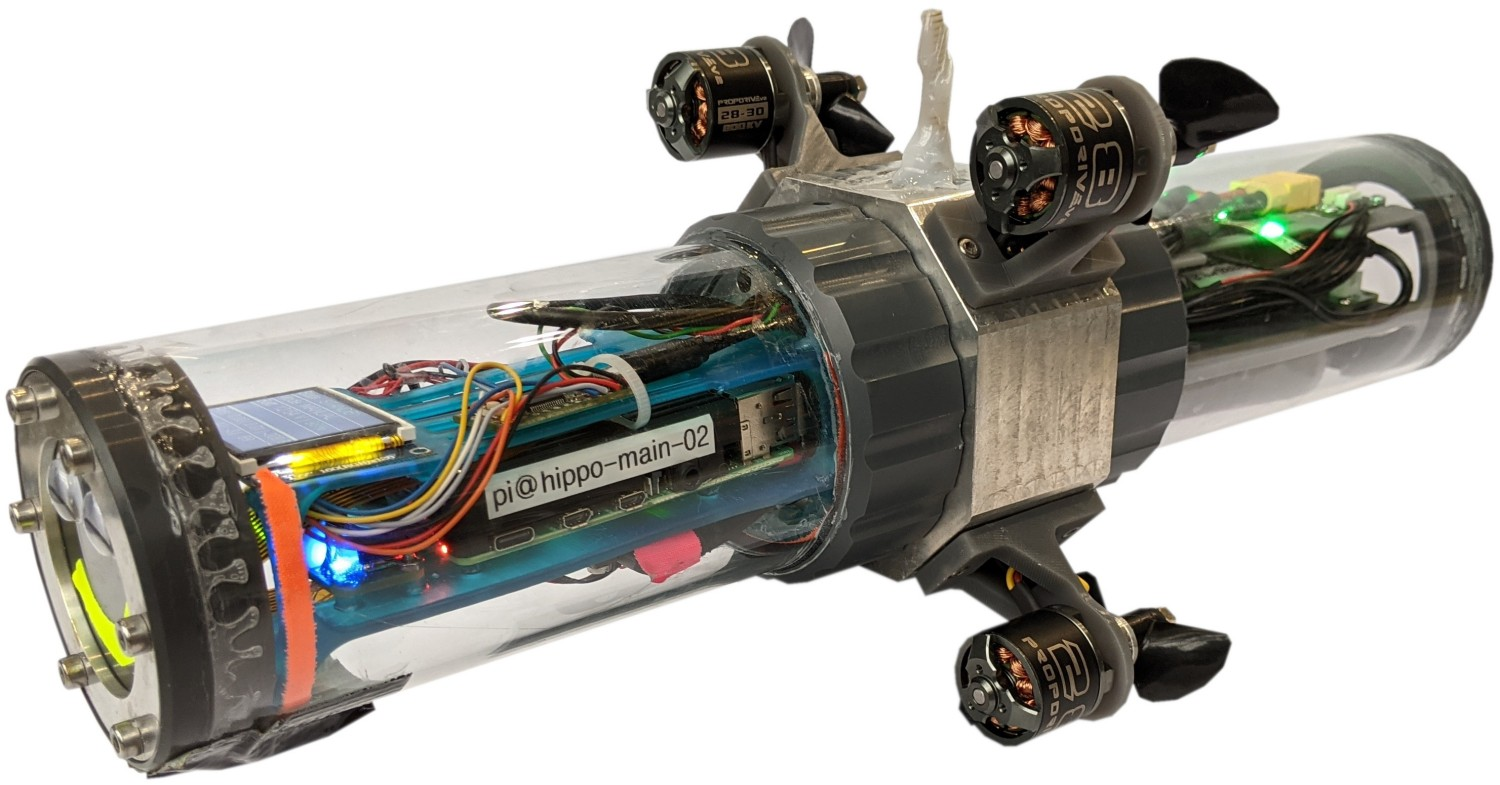
\includegraphics[width=0.4\textwidth]{hippo_picture}
    \quad\quad
    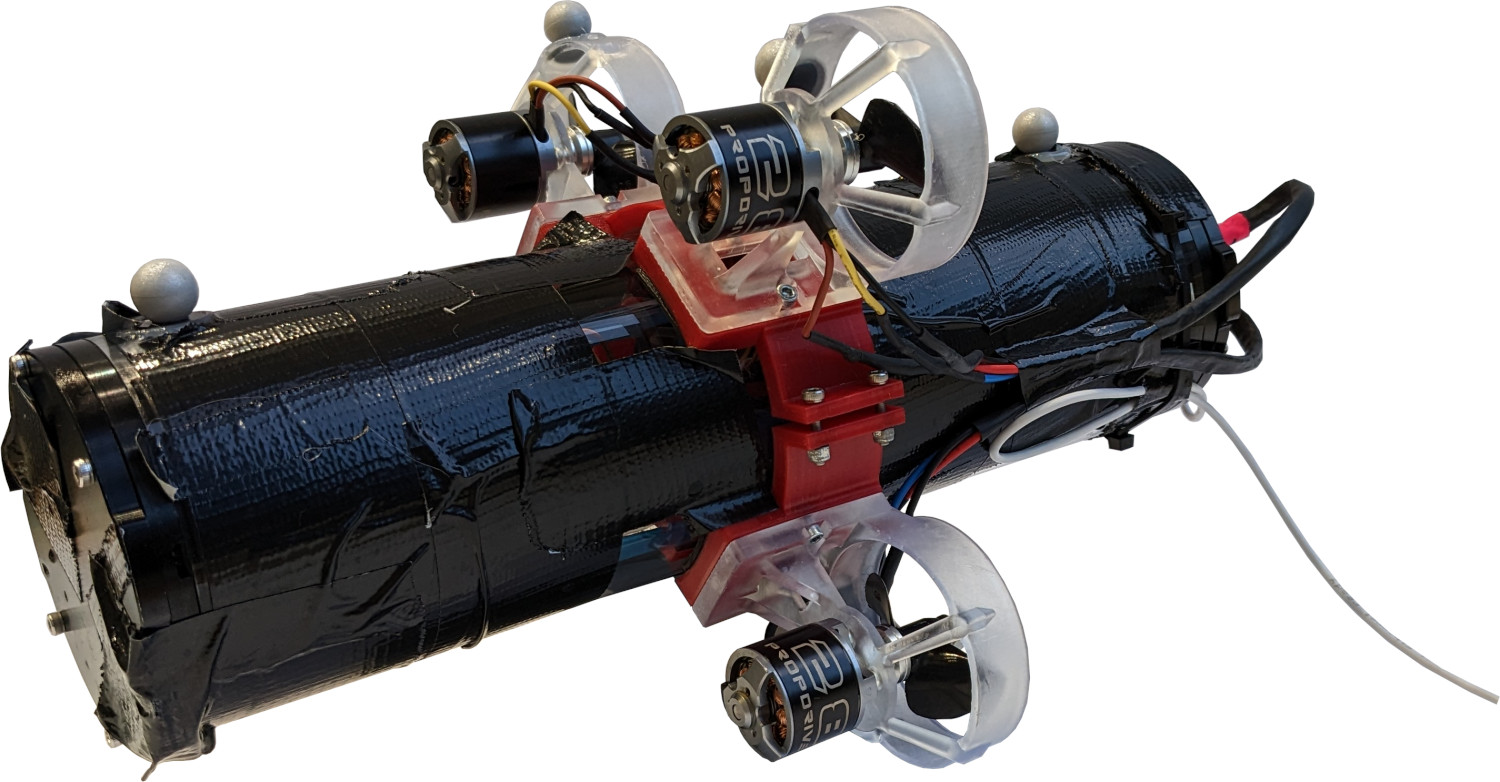
\includegraphics[width=0.4\textwidth]{hippo3_picture}
    \caption{\textcolor{blue}{HippoCampus $\mu$AUV in its heavy configuration (\textit{left}) and redesigned version based on BlueRobotics off-the-shelf components (\textit{right}).} \textcolor{red}{reference in text}}
    \label{fig:new-vehicle-design}
\end{figure}
In contrast to its predecessor it is built from off-the shelf components, with exception to the 3d-printed mounts for the electric components and motors. It weighs \unit[2.31]{kg} including additional ballast weight of approximately \unit[150]{g} to neutralize buoyancy.

Essential hardware components are the four thrusters, the \ac{fcu} and the onboard computer. The thruster configuration resembles those of quadrocopters. The x-configuration enables direct actuation of forward thrust and all three rotational degrees of freedom. Hence, HippoCampus is an underactuated but still highly agile underwater robot, due to its small size and low weight.

The \ac{fcu} is a PixRacer, usually used as flight controller \acp{auv}. It has an \ac{imu}, including an accelerometer, gyroscope and magnetometer, used for onboard state estimation. Low-level control loops are usually executed on the \ac{fcu}. High-level controls and mission planning tasks, as well as computational heavy operations such as image processing, are the responsibility of the onboard computer. The onboard computer is a Raspberry Pi 4B with an ARM A72 quad-core processor.

\subsection{Software Architecture}
The present general software architecture of the HippoCampus platform is shown in \Cref{fig:software-architecture-overview}. For a detailed description the reader may refer to \cite{duecker-phd}. 
\begin{figure}[h!]
	\centering
     \def\svgwidth{12cm}  
	\input{images/02/03_hippo_system_architecture_draft.pdf_tex}
	\caption{System architecture of the HippoCampus $\mu$AUV \cite{duecker-phd}.}
    \label{fig:software-architecture-overview}
\end{figure}
The modular design is divided into modules assigned to the \ac{fcu} and modules assigned to the onboard computer.
Two different frameworks are deployed, PX4 \cite{PX4} and \ac{ros} \cite{ros}.
Both are similar from the perspective that both frameworks implement a publish-subscribe pattern.
The interconnection between PX4's \ac{uorb} running on the \ac{fcu} and \ac{ros} on the onboard computer is realized via a combination of \ac{mavlink} \cite{mavlink} and MAVROS.
Since \ac{uorb} is restricted to intra-process communication, communication with external devices is done via \ac{mavlink}.
\ac{mavlink} is a communication protocol for \acp{uav}.
The interface between \ac{mavlink} and \ac{ros} is MAVROS. It is a bidirectional bridge, translating messages from \ac{mavlink} to corresponding \acs{ros}-messages and vice versa. This whole setup is depicted in \Cref{fig:ros-px4-communication}.
\begin{figure}[h!]
	\centering
    \def\svgwidth{12cm}  
	\input{images/02/03_sw_layer.pdf_tex}
	\caption{HippoCampus software architecture with multiple layers of abstraction according to \cite{duecker-phd}. Communication between \acs{ros} (left) and PX4 (right) via \acs{mavlink} and MAVROS.}
    \label{fig:ros-px4-communication}
\end{figure}
It is clear, that the communication between the onboard computer and the \ac{fcu} involves several layers of abstraction on multiple conversions of messages. This renders the communication more complex and less efficient. This can be overcome by migrating from \ac{ros} to its successor \ac{ros2}, that enables direct communication between the \ac{fcu} and the onboard computer via \ac{dds}. Hence, all software modules developed in the scope of this thesis are implemented using \ac{ros2}.

The interested reader may refer to \cite{ros2} for an exhaustive overview of the design and architecture of \ac{ros2}. The main aspects relevant for this thesis are listed below.

Embedded systems are well integrated into the \ac{ros2} framework. A \ac{ros2} stack specifically designed for microcontrollers, called micro-ROS, allows the direct communication between computers and microcontrollers. With regard to HippoCampus, this means the \ac{fcu} running PX4 and the onboard computer can communicate directly without the abstraction layers introduced by MAVROS and \ac{mavlink}. This enables high rate data streams between the devices.

Furthermore, \ac{ros2} introduces the concept of \ac{qos} as it relies on \ac{dds} for communication. Hence, data streams transporting sensor data can be declared to be transmitted with \emph{best effort}. As a result, the loss of messages is accepted, while the latency can be reduced. This especially useful for sensor data, where it is of interest to receive the most recent measurements as fast as possible. For message sizes of up to \unit[1]{MB} latencies below \unit[1]{ms} can be achieved for communication between different processes \cite{ros2}. High latencies impose delays on control loops and state estimation with possibly severe negative influence on their performance.

Though not required for this thesis, it should be noted, that \ac{ros2} is suitable for real-time systems. In contrast to its predecessor, \ac{ros2} can be configured for deterministic scheduling to enforce real-time constraints \cite{ros-realtime20}. This can be a critical property for the field of mobile robotics, where deterministic execution times can be safety critical.

\section{Review on Motion Planning}
\label{sec:review-motion-planning}
\subsection{Underwater Motion Planning}
\begin{itemize}
    \color{red}
    \item \cite{Panda20} for review on auv path planning
\end{itemize}
\label{sec:underwater-motion-planning}
We refer to motion planning as either path planning or trajectory planning. Path planning only considers the spatial aspect of motion, while for trajectories there is a relation between the geometric path and time. Often, it is convenient to decouple the path planning aspect from the temporal planning. By assigning a velocity profile to the planned path, a trajectory can be obtained after the path planning problem is solved. Hence, no rigorous distinction between trajectory and path planning is made in the course of this section.

In the following, a selection of widely used algorithms for solving underwater path planning problems is introduced, their concept briefly summarized and example applications in the domain of \acp{auv} presented. This should provide a sufficient overview of the state of the art, to discuss strengths and limitations of existing underwater path planning methods.

\cite{Panda20} presents a comprehensive overview of various path planning approaches for single- or multi-\acsp{auv} scenarios. Since multiagent systems are not the focus of this thesis, the interested reader may refer to \cite{Panda20} for more information on this topic.

%  \cite{Gomez15} classifies different path planning methods: geometric methods, graph- and tree-based methods and artificial potential fields methods. For this thesis, the categorization by the used techniques seems less useful than grouping the methods by their field of application.

\subsubsection{Graph- and tree-based Methods}
According to \cite{Gomez15}, methods falling in this category are subject to the highest research effort during recent years. Well known and often used algorithms belong to this group of path planning methods, such as A*, \ac{rrt} or \ac{fmm}.


\paragraph{Grid-based Search}
For grid-based approaches like A*, the vehicle states or the environment are discretized and encoded as nodes in a graph, building the search space. Costs are assigned to the edges connecting the nodes. Depending on the used algorithm, a path is searched, that connects the initial state with a desired goal state.
To obtain, for example, the shortest path, the costs can be defined as the euclidean distance between discrete positions in the environmet. The  nodes of the graph encode the discretized environment.
Subsequently, a search algorithm guaranteeing optimality can be deployed to find the path with the lowest costs, if one exists. Due to dicretization, accuracy is decreased. A smaller grid size counteracts this problem, but increases the search space and therefore the computational costs for finding a solution.

The authors in \cite{Fernandes2015TowardsAO} declare A* in its generic form as general not suitable for mobile robots with time constraints, due to the performance costs associated with traversing the state space if replanning is required. Still, there exist various publications applying variants of A* in the context of path planning for mobile robots and \acp{auv} in particular.

Applications of A* in the domain of \acp{auv} go back to the 90s \cite{Carroll92}, while still being extended in recent works \cite{zhang20}. Common to these approaches is the application for oceanic environments, where obstacles are assumed to be static, traveled distances to be large, and vehicle dynamics not to be relevant. The main focus often lies on considering ocean currents for path planning.

Another algorithm used for grid-based search is \ac{fmm}. The principle of \acs{fmm}-based path planning is based on simulated wave propagation in order to obtain distance fields. Obstacles in the environment can be taken into account and in case of constant propagation the optimal path between start and goal position in terms of distance can be found. Modifications to the wave propagation can be used to compute paths with different requirements.

The authors in \cite{Petres09} present a modification of \ac{fmm} called \acs{fmm}*. They exploit the reduced computation due to an appropriate heuristic function to solve path planning problems in dynamic environments, i.e. the environment changes or is partially unknown. They observe improved performance regarding computation time compared to A*. Additionally, they were able to enforce curvature constraints for the planned path.

\paragraph{Sampling-based Search}

A typical representative of sampling-based methods is \ac{rrt}. Even though, the original version of \ac{rrt} does not provide optimality, it compensates for that by being able to efficiently solve complex planning problems, that are possibly high-dimensional \cite{Devaurs16}. Randomly sampled points are connected to generate a tree to find a path between initial and goal state.

In \cite{Young13} the authors present a path planning approach based on \ac{rrt} for \acp{auv} in the presence of obstacles. Kinematic constraints, such that the vehicle can only move with certain velocity limits are respected. A model for the hydrodynamic properties of the vehicle is not considered, though.

The problem of non-optimality is addressed in \cite{Karaman11} with a modification of \ac{rrt}, called anytime \ac{rrt}, though not applied in the underwater domain. The idea is, to find a solution as fast as possible and improve the solution if given further computation time. This renders the approach especially useful for dynamic environments.

An informed variant of \ac{rrt}, called RRT*, is used in \cite{Ma18} for terrain-aided navigation for long range navigation of \acp{auv}.

\subsubsection{Artifical Potential Fields}
It the basic idea of path planning is to model the robot as electric charge \cite{Gomez15}. Obstacles are represented by charges with the same sign. Hence, the robot is repelled from the obstacles. The goal state is modeled as charge with opposite sign and therefore attracts the robot. To find a way to the goal, the path minimizing the energy of the robot is searched, which can be accomplished by following the steepest gradient. The main drawback of this method is, that it is not guaranteed, that the robot is not trapped inside a local minimum. 

An improvement over the basic method of potential fields in the context of path planning for \acp{auv} is presented in \cite{Fu-guang05}. The authors suggest a heuristic to escape the local minimum in the vicinity of concave obstacles.

\subsubsection{Model Predictive Control}

Though, actually a control and not a path planning method, model predictive control can still be used for path planning problems, as will be presented below. In model predictive control methods the future state of a robot is predicted, based on a dynamic model of the robot. The future states depend on system inputs. By defining a cost function, an optimal solution regarding the control inputs to reach a desired state can be computed. To close the feedback loop, this optimization is performed at every time step. Hence, external disturbances and model inaccuracies are considered. But this implies one of the major disadvantages of this method, as the computation of the optimal solution in each time step is usually computational expensive.

Model predictive control in the area of path tracking for \acp{auv} has been presented in \cite{Shen16}. The authors use a multi-objective model predictive control framework and prove the validity of their approach in a simulation of the Saab SeaEye Falcon. In \cite{Heshmati18} a waypoint-tracking controller, implemented as nonlinear model predictive control, is proposed. The presented control scheme considers ocean currents, thruster saturation, velocity limits and incorporates obstacle avoidance. The latter proves this approach to be a promising for low level maneuvering. The waypoints can be provided by a high level mission planner and the model predictive controller is responsible for reaching them without violating the constraints.


\subsubsection{Discussion}
\begin{itemize}
    \color{red}
    \item Vehicles are large/slow
    \item Have more computational power or algorithm in general not real timecapable.
\end{itemize}

We observe, that the problem of path planning for \acp{auv} has usually been examined for traditional \acp{auv}, operating in ocean environments.
Hence, the publications often focus problems characteristic for the marine domain.
Ocean currents are considered of higher priority than accounting for the vehicle dynamics.
Since traditional \acp{auv} are very heavy and slow in relation to their size, it is questionable whether path planning approaches for this type of vehicles would be directly transferrable to the domain of hydrobatic \acp{uauv}, anyway \cite{hydrobatic}.

Furthermore, many approaches solve the problem for static environments, as it is usually assumed when deploying A*-based concepts. This is reasonable, if mainly the geometric restrictions caused by the coastal line and constant ocean currents are of concern. As a consequence, these algorithms cope with dynamic changes and replanning rather badly.

\subsection{Review on Agile Path Planning Methods}
In this section a brief review on agile path planning methods is given. As the previous section on path planning for \acp{auv} indicated, the problem of \emph{agile} path planning is underrepresented in the literature. Hence, in this section the review is extended on the aerial domain. Due to the similarity in the design of small-scale \acp{uav} and \acp{uauv}, it is likely that findings in the aerial domain can be transferred to the area of hydrobatic \acp{uauv}.

In \cite{MellingerKumar11} the authors present a minimum snap trajectory generation method for quadrocopters. This approach is demonstrated to be real-time capable. The trajectory is defined by \emph{keyframes}, i.e. a position and a yaw angle, and corridor constraints between keyframes, as seen in \Cref{fig:mellinger}.
\begin{figure}
    \centering
    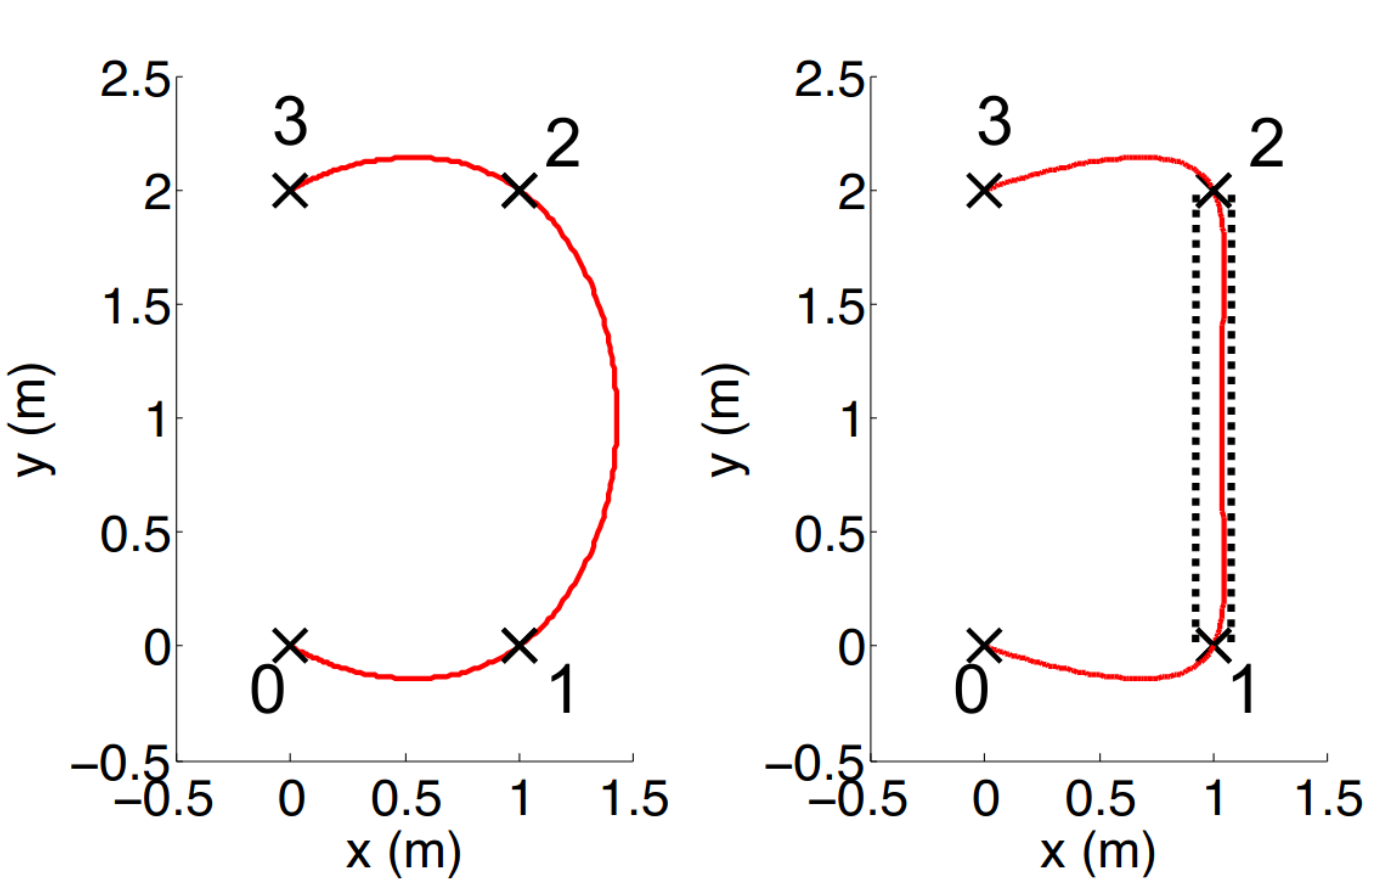
\includegraphics[width=0.6\textwidth]{images/02/mellinger.png}
    \caption{$xy$-plot of a minimum snap trajectory with keyframes depicted as crosses. On the left the trajectory has no corridor constraints, on the right the corridor constraint is visualized as dotted rectangle \cite{MellingerKumar11}.}
    \label{fig:mellinger}
\end{figure}
The capability of this approach is demonstrated in experiments, where the quadrocopter was able to fly through a thrown circular hoop, reaching velocities of \unit[3.6]{m/s}.

A combination of minimum snap trajectories and \ac{rrt} is presented in \cite{Richter16} and \cite{Shi20}.
\ac{rrt} is used as a high-level planner whereas the minimum snap trajectory generator is used to compute smooth trajectories suitable for the dynamics of \acp{uav}. 
The authors try to deal with the challenges of indoor navigation and use \ac{rrt} to generate waypoints as piecewise linear path to reach a goal position in presence of a cluttered environment. Subsequently, the waypoints are connected smoothly by minimum jerk trajectories.
The implementation sacrifices the asymptotical optimality of \ac{rrt}* in favor of dynamically more suitable paths and reduced computation time. Even tough, the computation time could be reduced by a factor of 40, the remaining computation time is still in the magnitude of several seconds. Hence, the approach is not able to account for dynamic obstacles.


\begin{itemize}
    \color{red}
    \item Natural to look at quadrocopters to transfer solutions to the underwater domain because of the similarity of the design.
\end{itemize}
\subsection{Discussion}


% \begin{landscape}
\begin{table}[]
%\renewcommand{\arraystretch}{1.0}
    \caption{Overview on ....}
		%\hspace*{-1.5cm}  % move table down (left in landscape) - tabular width: 
		\centering
		% change column width: >{\hsize=1.5\hsize\linewidth=\hsize}
		% >{\hsize=0.5\hsize\linewidth=\hsize}
		\begin{NiceTabular}
            {
            %%%%% Leider scheint die beste Methode wirklich hardgecodete Spaltenbreiten zu sein - hier am Ende rumspielen
            >{\scriptsize\arraybackslash}m{1.7cm} % Method
            >{\scriptsize\centering\arraybackslash}m{1.2cm} % 
            >{\centering\scriptsize\arraybackslash}m{1cm}   %
            >{\centering\scriptsize\arraybackslash}m{3cm}   % 
            >{\centering\scriptsize\arraybackslash}m{2cm}   % 
            >{\centering\scriptsize\arraybackslash}m{3.2cm} % 
            }
            \toprule
            %%%%%%%%%%% Top row - names of each columns
            Example
            &  Domain
            &  Method
            & Optimality
            & Obstacle Avoidance
            & Comment \\  
            \midrule 
            
            %%%%%%%% Beispiel
            \cite{Carroll92}
            & underwater
            & A*
            & yes (cost not defined)
            & static
            & Considers static ocean currents and static spatial constraints.
            \\ 

            \cite{zhang20}
            & underwater
            & A*
            & distance
            & static
            & Improvement of computation efficiency for real-time path planning.
            \\

            \cite{Petres09}
            & underwater
            & \ac{fmm}*
            & yes (implementation dependent)
            & dynamic
            & Combination of A* and \ac{fmm}. Path curvature can be constrained and partially replanning in case of dynamic changes is possible.
            \\

            \cite{Young13}
            & underwater
            & \ac{rrt} and A*
            & no
            & dynamic
            & \ac{rrt} generates obstacle free path with kinematic constraints. Shortest available path searched with A*. Not optimal, though.
            \\

            \cite{Karaman11}
            & land
            & anytime \ac{rrt}*
            & distance (asymptotically)
            & static
            & Obstacles are considered static. Solution is dynamically refined during movement after initial solution has been found.
            \\

            \cite{Ma18}
            & underwater
            & \ac{rrt}*
            & distance (asymptotically)
            & static
            & The terrain is considered as obstacle and therefore static. Online replanning is possible.
            \\

            \cite{Fu-guang05}
            & underwater
            & Potential Fields
            & none
            & dynamic
            & Avoids local minima problem inherent to the potential fields method for concave obstacles.
            \\

            \cite{Heshmati18}
            & underwater
            & \acs{mpc}
            & energy
            & static
            & Exploits ocean currents to minimize energy consumption.
            \\

            \cite{MellingerKumar11}
            & aerial
            & minimum snap polynomial
            & snap
            & dynamic (indirect)
            & Highly aggressive maneuvers possible. Obstacle avoidance can be accomplished indirectly by setting appropriate constraints.
            \\
            
            \cite{Richter16}\cite{Shi20}
            & aerial
            & \ac{rrt} + minimum snap
            & not globally
            & static
            & No global optimality in favour of computation time, reduced from minutes to seconds. Respecting vehicle dynamics.
            \\
            \bottomrule
		\end{NiceTabular}
		\label{tab:state_of_the_art}
\end{table}
% \end{landscape}

